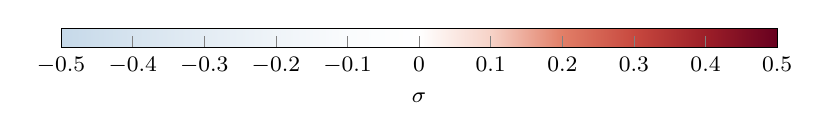
\begin{tikzpicture}
\begin{axis}[
hide axis, scale only axis,
width=0.75\textwidth, height=0pt,
colormap={sigmamap}{rgb(0.0000)=(0.7760,0.8510,0.9140); rgb(0.1000)=(0.8392,0.8918,0.9369); rgb(0.2000)=(0.8913,0.9259,0.9563); rgb(0.3000)=(0.9374,0.9569,0.9743); rgb(0.4000)=(0.9799,0.9861,0.9917); rgb(0.5000)=(1.0000,0.9999,0.9999); rgb(0.6000)=(0.9659,0.8254,0.7818); rgb(0.7000)=(0.8840,0.4951,0.4053); rgb(0.8000)=(0.7820,0.2849,0.2466); rgb(0.9000)=(0.6131,0.1208,0.1566); rgb(1.0000)=(0.4040,0.0000,0.1220)},
point meta min=-0.5, point meta max=0.5,
colorbar horizontal,
colorbar style={
  width=0.75\textwidth, height=7pt,
  at={(0,0)}, anchor=north west,
  xlabel={$\sigma$},
  xlabel style={font=\footnotesize},
  tick label style={font=\footnotesize},
  xtick pos=bottom,
},
]
\addplot[draw=none] coordinates {(0,0)};
\end{axis}
\end{tikzpicture}
